% -- Encoding UTF-8 without BOM
% -- XeLaTeX => PDF (BIBER)

\documentclass{cv-style}     % Add 'print' as an option into the square bracket to remove colours from this template for printing.

\setdefaultlanguage{french}
\sethyphenation{french}{} % Add words between the {} to avoid them to be cut

%----------------------------------------------------------------------------------------
%	Page layout
%----------------------------------------------------------------------------------------
\cvheadheight{3.5cm}
\cvasidewidth{4.7}
\cvasidevpos{3.5}
\cvmainwidth{11.5cm}
\geometry{left=6.4cm, top=2.5cm, right=1cm, bottom=1cm}


%----------------------------------------------------------------------------------------
%	hyperlink setup
%----------------------------------------------------------------------------------------
\hypersetup{
    pdftitle=CV \textbar{} Laura Gomez,%
    pdfauthor=Laura Gomez
}

%----------------------------------------------------------------------------------------
%	Setup las updated text
%----------------------------------------------------------------------------------------
%\lastupdated{Mise à jour le \today}

%----------------------------------------------------------------------------------------
%	Add a few custom packages
%----------------------------------------------------------------------------------------
\usepackage{fontawesome}

\begin{document}

\header{Laura }{Gomez}{Tecnical Project Manager in Mechatronics and Biomechanics}         % Your name
%\lastupdated

%----------------------------------------------------------------------------------------
%	SIDEBAR SECTION  -- In the aside, each new line forces a line break
%----------------------------------------------------------------------------------------

\begin{aside}
    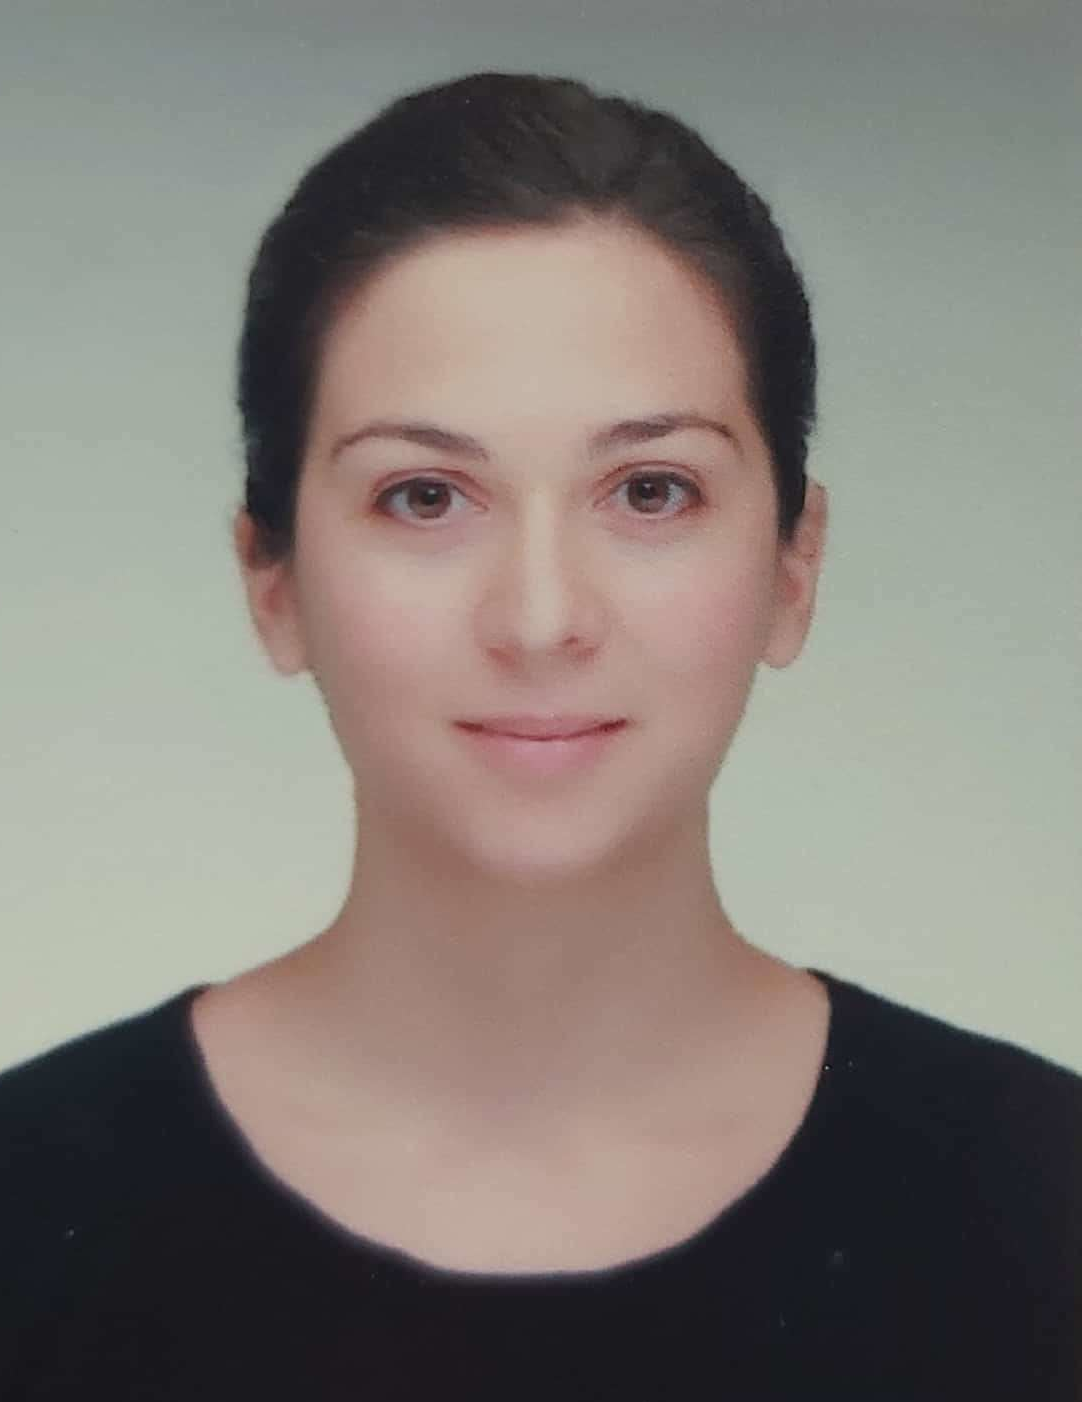
\includegraphics[width=.8\columnwidth]{img/LG}
    %\textbf{Immediate availability}
    91 rue du Colonel Fabien
    92160 Antony
    France
    ~
    French Nationality
    13 January, 1989, France
    In cohabitation
    Driving licence
    %
    \section{Contact}
    laura-gomez@gmx.fr
    +33 7 70 49 23 44    
    %
    \section{Project Management}
    Microsoft Office
    ERP (Dolibarr, Sage)
    Requirement management (IBM DOORS, Reqtify)
    ~
    Drafting patent
    Follow-up Regulatory marking
    Follow-up of technical documentation
    %
    \section{Programming}
    C, Matlab
    Embedded systems %(Arduino, Mbed)

    CAD %(Solidworks, Fusion360, OpenSim)

    Multiphysics simulation %(Flotherm)
    Electronic design  %(Simulink, Labview, Zuken, Altium) 
    Human movement study %(Nexus pour Vicon, MT Manager pour Xsens (centrales inertielles))
    %
    \section{Languages}
    French (maternal language)
    English (fluent)
    Spanish (fluent)
    %
    \section{Soft Skills}
    Autonomous and proactive
    Analytical thinking
    Good team player
    %
    \section{Hobbies}
    Cello and orchestra
    Cycling and running
    %
\end{aside}

\section{Abs}{tract}

As a mechatronics engineer, I had the opportunity to drive the hardware and software development of products,
from their development phase to their industrialization. I was also given the opportunity to manage the compliance of products
that already existed so that they could meet the specific needs of the client.
In this context, I ensured good communication between all internal and external stakeholders concerned,
in order to meet the deadlines and the quality of the final product.
Highly adaptable, I enjoy learning on a daily basis and sharing my knowledge with my colleagues.

\section{Professional }{Experience}

\begin{entrylist}
%------------------------------------------------
\entry
  {2021}
  {NeoFarm}
  {Farming robot}
  {\jobtitle{Mechatronics Engineer, Industrial Engineer}\\
  Development and testing of farming tools adapted to the robot

  Vendor Tracking

  Regulatory marking tracking

  ERP implementation and design rules
   }
 
%------------------------------------------------
\entry
  {2020}
  {Safran}
  {Defence}
  {\jobtitle{System engineer}\\
  Biomechanical study

  Collection and synthesis of the need from multiple stakeholders

  Search for existing solutions in the market

  French and foreign supplier monitoring

  Application of requirements under IBM DOORS
  }
%------------------------------------------------
\entry
  {2018--2019}
  {Safran - Zodiac (consultant for Alten)}
  {Aeronautics}
  {\jobtitle{Mechatronics Systems Technical Project Manager}\\
  Collection of the needs of an Italian customer

  Translation of the need into R\&D actions

  Management of technical and documentary exchanges between the client and the various R\&D teams

  Harness design with Zuken, working with the Production team

  Customer System Testing
 
  }
%------------------------------------------------
\entry
 {2017--2018}
 {Air Liquide Medical System (consultant for Ametra)}
 {Medical - ventilation}
 {\jobtitle{Mechanical referent - new product and plastics processing}\\
 In charge of the evolution of the current system to reduce cracks

 Follow-up of initial samples of the plastic shell of a new device

 Follow-up of plastic manufacturers

 8D
 }
%------------------------------------------------
\entry
 {2016}
 {CEA (consultant for Manpower)}
 {Food processing industry cobotics}
 {\jobtitle{Technical project manager of cobotic systems}\\
 Study of the need at the workplace (biomechanical)

 Solution search, design, demonstrator manufacturing

 Testing of prototypes by operators

 Drafting of patents
 }
%------------------------------------------------

\end{entrylist}

%----------------------------------------------------------------------------------------
%	EDUCATION SECTION
%----------------------------------------------------------------------------------------

\section{Educ}{ation}

\begin{entrylist}
%--------------------------------------G----------
\entry
{2013--2015}
{Master of Research in Biomedical Engineering {\normalfont biomechanical specialty}}
{BME et Arts et Métiers, France}
{International Master's}
%------------------------------------------------
\entry
{2008--2013}
{Mechatronics Engineering School {\normalfont Robotics and Simulation Specialties}}
{ISTY - UVSQ, France and Korea}
{6 months in Korea at Ajou University}
\end{entrylist}

\end{document}
